Memoization is the practice of storing previously computed values of a function so that future calls with the same inputs can be evaluated by lookup rather than re-computation.
To transfer this idea to probabilistic programming, we now introduce a language construct called a
\emph{statistical memoizer}.  Suppose we have a function $\ftt$ which can be evaluated 
but we wish to learn about the behavior of $\ftt$ using as
few evaluations as possible.  The statistical memoizer, which here we give the
name \gpmem, was motivated by this purpose.  It produces two outputs:
\[ \ftt \xrightarrow{\gpmem} (\ftt_{\text{compute}}, \ftt_\emu). \]
The function $\ftt_{compute}$ calls $\ftt$ and stores the output in a memo
table, just as traditional memoization does.  The function $\ftt_\emu$ is
an online statistical emulator which uses the memo table as its training
data.  A fully Bayesian emulator, modelling the true function $\ftt$ as a
random function $f \sim P(f)$, would satisfy
\[
\texttt{(}\ftt_\emu\ \xtt_1\ \ldots\ \xtt_k\texttt{)}
\sim
P\pn{
  f(\xtt_1), \ldots, f(\xtt_k)
  \mvert
  \text{$f(\xtt) = \texttt{(f x)}$ for each $\xtt$ in memo table}
}.
\]
Different implementations of the statistical memoizer can have
different prior distributions $P(f)$; in this paper, we deploy a \ac{GP} 
prior (implemented as \texttt{gpmem} below).  Note that we require the ability
to sample $\ftt_\emu$ jointly at multiple inputs because the values of
$f(\xtt_1),\ldots,f(\xtt_k)$ will in general be dependent.


\begin{figure}
\noindent\centering
% for double arrows a la chef
% adapt line thickness and line width, if needed
\begin{tikzpicture}[thick]
\node[] (start) {};
 \node[draw,circle,minimum size=1.5cm,left = 0.5cm of start] (f) {f$_{\text{compute}}$};
 \node[draw,right = 0.5cm of start,circle,minimum size=1.5cm] (K) {$\mathbf{K}_{\theta}$};
 %\node[below left of=f_K,xshift=-1.7cm,yshift=-0.1cm] (theta) {$\bm{\theta} \sim P(\bm{\theta})$};
 \node[draw,rectangle,below=1.5cm of start, text width = 6.6cm] (gpmem) {\centering\texttt{gpmem}\vspace{2mm}
 
\small$\text{memo table} = (\mathbf{x}_{past},\mathbf{y}_{past})$\vspace{1.5mm}
 
 
\small$P(f_{emu}(x) \mid \mathbf{x}_{past},\mathbf{y}_{past})\sim \mathcal{N}(\mu(\mathbf{x}),\mathbf{K}_\theta\big(\mathbf{x},\mathbf{x})\big)$
 };
%  \node[draw,rectangle,color=ForestGreen,below = .1ex of gpmem,minimum width=1.5cm, minimum height=0.4cm,yshift=0.9cm,xshift=0.3cm] (mark) {};
  \node[draw,rectangle,dashed,right=2.2cm of K, text width = 2.2cm] (math) {\small
 $\mathbf{K}_{\theta} = \text{SE}(x,x^\prime)$\vspace{1.5mm}
 
 $\theta \;\;\,\,= \{sf,\ell \}$\vspace{1.5mm}
 
 $sf\;\, \sim P(sf)$\vspace{1.5mm}

 $\ell\;\;\;\; \sim P(\ell)$\vspace{1.5mm}
 
 
%\scriptnotesize
%
%%$\mu(\mathbf{x}) =\mu(\mathbf{x}) + \mathbf{K}_\theta(\mathbf{x},\mathbf{x}_{past})\mathbf{K}_\theta(\mathbf{x}_{past},\mathbf{x}_{past})^{-1}(\mathbf{y}_{past} - \mu(\mathbf{x}_{past}))$
 };
 \node[draw,rectangle,dashed,minimum size=1cm,left= 2.2cm of f] (resources) {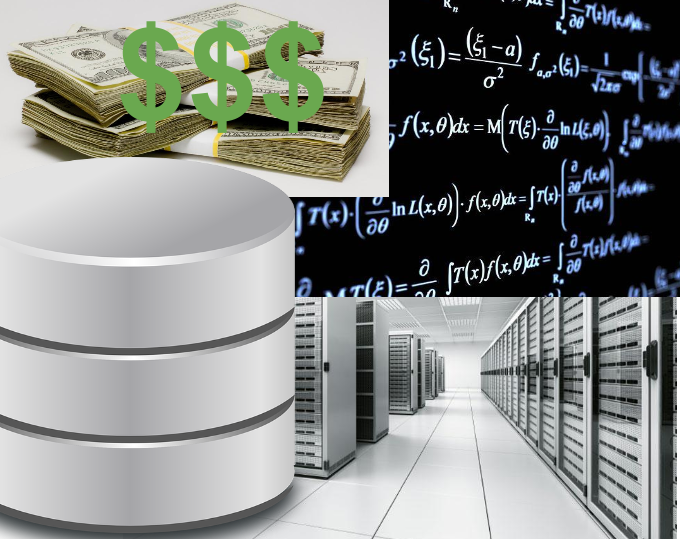
\includegraphics[width=3cm]{figs/resources.png}};

\node[draw,rectangle,below=1cm of gpmem,text width =7cm] (f_emu) {\centering $f_{emu}$ \vspace{2mm}

\begin{tabular}{l|l}\small
  $x$ & $f(x)$ \\ \hline
   $x_1$  & $y_1$ \\ 
   $x_2$  & $y_2$ \\
  $\cdots$ &   $\cdots$
 \end{tabular}
 $\;\;\;\;$
 \begin{tabular}{l}
 Parameters:\\
\small  Kernel lengthscale $\ell$  \\
\small Kernel scale-factor $sf$
 \end{tabular}

};
%\node[right = 1.2 cm of f_emu,inner sep = 0pt,outer sep=0pt,minimum size=25pt] (emu_annotate) {Infer: $\theta\;$};

\node[below = .1ex of gpmem,inner sep = 0pt,outer sep=0pt,xshift=-0.3cm] (helper1) {};
\node[below = .1ex of gpmem,inner sep = 0pt,outer sep=0pt,xshift=0.7cm] (helper2) {};

\node[above = .1ex of f_emu,inner sep = 0pt,outer sep=0pt, xshift=0mm] (helper_emu) {};

\node[above = 0.75cm of resources,inner sep = 0pt,outer sep=0pt] (helper_resource_top) {};
\node[left = 1cm of f_emu] (x_hat) {$\hat{x}$} ;
\node[right = 1cm of f_emu] (GaussianHat) {$\mathcal{N}(\hat{\bm\mu},\hat{\mathbf{K}})$} ;

%\node[right =1. cm  of f_emu, yshift=1.5cm] (infer) {\small Infer: $\ell$, $sf$} ;

% 1st pass: draw arrows

  \draw[thick,dashed,->] (resources) --node [pos=0.5,below] {resource}  node [pos=0.5,above] {outside} (f);
  \draw[thick,dashed,->] (math) -- node [pos=0.5,above] {Kernel} (K);
  \draw[thick,->] (K) -- (gpmem);
  \draw[thick,->] (f) -- (gpmem);
 % \draw[thick,->] (theta) -- (gpmem);
  \draw[thick,->] (gpmem) -- (f_emu);

 % \draw[thick,->,color=ForestGreen] (helper_compute) -- node[pos=0.5, sloped, below] {probe} (helper1);
 % \draw[thick,->,color=ForestGreen] (helper2) -- node[pos=0.5, sloped,above] {improves} (helper_emu);
   % \draw[thick,->,dashed,color=ForestGreen] (helper_resource) -- node[pos=0.5,above] {$f_{com}(x_2)=y_2$} (f_compute);
  %  \draw[thick,->,dashed,color=ForestGreen] (helper_resource) -- (resources);
     \draw[thick,->,dashed] (x_hat) -- (f_emu); 
     \draw[thick,->,dashed] (f_emu) -- (GaussianHat); 
 % \draw[thick,->] (theta) -- (gpmem);
  
   
%\path[](f_emu) edge [in=90, out=50,thick] (emu_annotate)
%    (emu_annotate) edge [->,in=310, out=270,thick]  (f_emu);
  % Note: If you have no branches, the 2nd pass is not needed

\end{tikzpicture}


\begin{tabular}{ll}
% line 1
& \\
\hline
\begin{lstlisting}[mathescape,escapechar=\#]
define f = proc( x) {
		    exp(-0.1*abs(x-2))) *
		    10* cos(0.4*x) + 0.2
		    }    
assume (f_compute f_emu) =  gpmem( f, K)
sample f_emu( array( -20, $\cdots$, 20)) 

\end{lstlisting}
& \raisebox{-0.5\height}{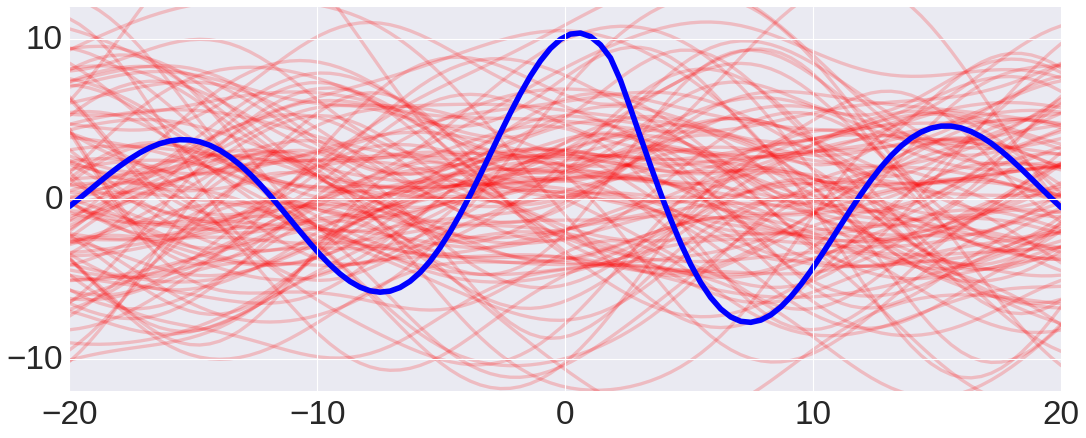
\includegraphics[height=2.5cm]{figs/tutorial_1.png}} \\ \hline
% line 2
\begin{lstlisting}[mathescape,escapechar=\#]
predict f_compute( 12.6)

sample f_emu( array( -20, $\cdots$, 20)) 

\end{lstlisting}
 &  \raisebox{-0.5\height}{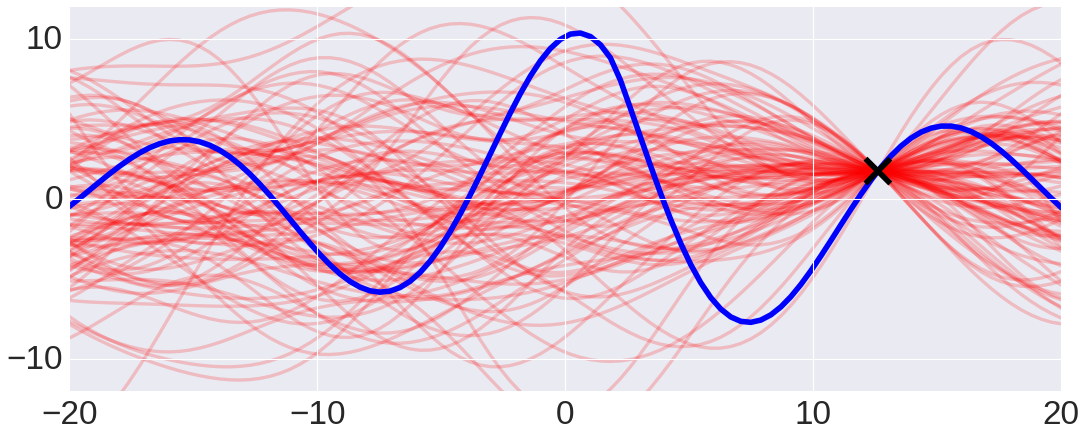
\includegraphics[height=2.5cm]{figs/tutorial_2.png}}  \\ \hline
% line 3 
 \begin{lstlisting}[mathescape,escapechar=\#]
predict f_compute( -6.4)

sample f_emu( array( -20, $\cdots$, 20)) 

\end{lstlisting}
 &  \raisebox{-0.5\height}{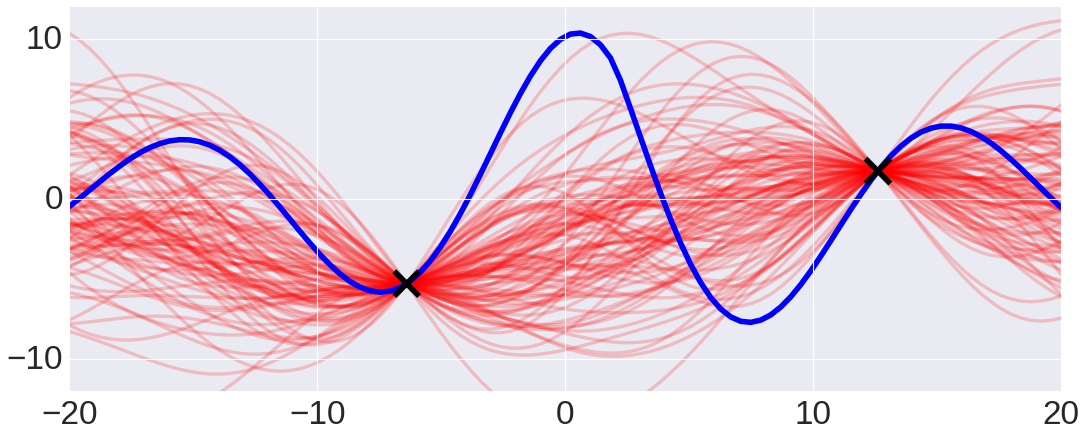
\includegraphics[height=2.5cm]{figs/tutorial_3.png}}  \\ \hline
% line 4
 \begin{lstlisting}[mathescape,escapechar=\#]
observe f_emu( -3.1) = 2.60 
observe f_emu( 7.8) = -7.60  
observe f_emu( 0.0) =  10.19

sample f_emu( array( -20, $\cdots$, 20)) 
  
\end{lstlisting}
 &   \raisebox{-0.5\height}{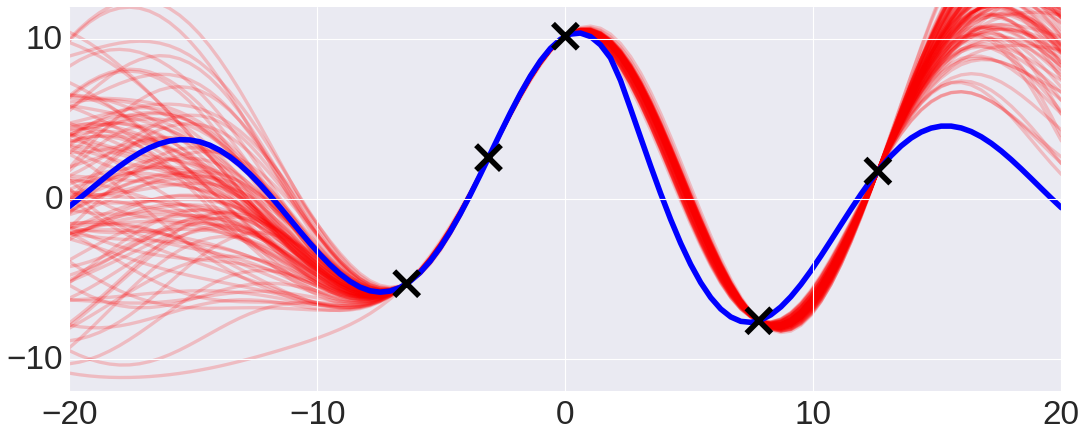
\includegraphics[height=2.5cm]{figs/tutorial_5.png}} \\ \hline
% line 5
 \begin{lstlisting}[mathescape,escapechar=\#]
infer mh(quote(hyper-parameter), one, 50)

sample f_emu( array( -20, $\cdots$, 20)) 
  
\end{lstlisting}
 &   \raisebox{-0.5\height}{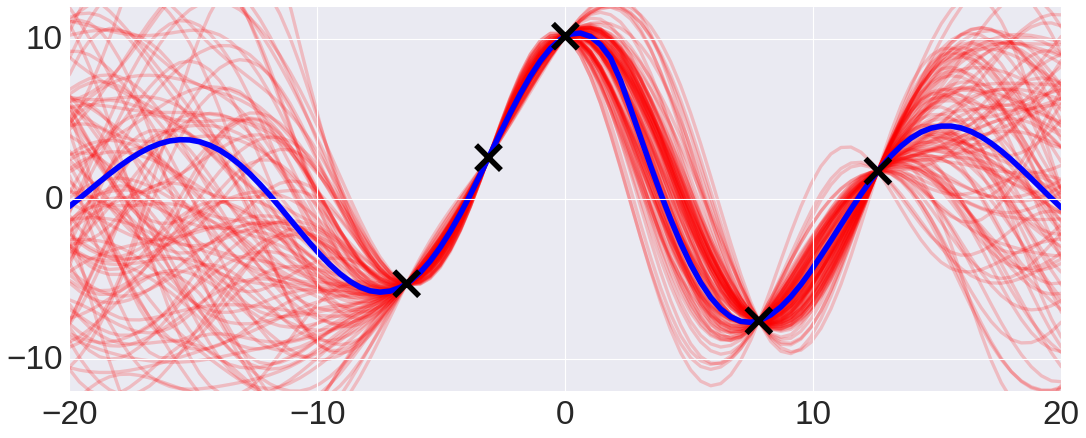
\includegraphics[height=2.5cm]{figs/tutorial_6.png}}
\end{tabular}
\captionsetup{aboveskip=-3pt}
\caption{\footnotesize \gpmem\ tutorial. The top shows a schematic of \gpmem.
  \texttt{f\_compute} probes an outside resource.
  This can be expensive (top left).
  Every probe is memoized and improves the emulator. Below the schematic we see the evolution
  of \gpmem's state of believe of the world given certain Venture
  directives. On the right, we depict the true function (blue), samples from the
emulator (red) and incorporated observations (black).}
\label{fig:gpmem_tutorial}
\end{figure}

% Panel 1
We explain how \gpmem, the statistical memoizer with \ac{GP}-prior, works using a simple tutorial
(Fig. \ref{fig:gpmem_tutorial}). 
The top panel (Fig. \ref{fig:gpmem_tutorial}, (a)) of this figure sketches the schematic of \gpmem.
$\ftt$ is the external process that we memoize. It can be evaluated using resources that potentially come
from outside of Venture.  
We feed this function into \gpmem\ alongside
a parameterised kernel $k$.  
In this example, we make the qualitative assumption of $f$ being smooth, and define
$k$ to be a squared-exponential covariance function:
\[
k = \kse = \sigma^2 \exp(-\frac{(x-x^\prime)^2}{2\ell^2}).
\]
The hyper-parameters $\thetabf$ for this kernel are sampled from a 
prior distribution which is depicted in the top right box.
Note that we annotate $\bm{\theta}=\{\texttt{sf},\texttt{l}\}$ for subsequent
inference as belonging to the scope ``hyper-parameters".

\gpmem\ implements a memoization table, where all previously
computed function evaluations ($\{\xbf,\ybf\}$) are stored. We also initialize a \ac{GP}-prior that
will serve as our statistical emulator:
\[
P(f_{emu}(x) \mid \xbf,\ybf,\thetabf)\sim
\mathcal{N}\big(\mupost,\Kpost)\big)
\]
where 
\[
P(f_{emu}(x) \mid \mathbf{x},\ybf,\thetabf) = \yprime 
\]
under the traditional \ac{GP} perspective.
All value pairs stored in the memoization table ($\text{memo table} = (\xbf,\ybf)$) are incorporated as observations of
the \ac{GP}.
We simply feed the regression input
into the emulator and output a predictive posterior Gaussian distribution determined by the \ac{GP} and
the memoization table.

% Panel 2
We can either define the function f that serves as as input for \gpmem\
 natively in Venture
(as shown in the Fig. \ref{fig:gpmem_tutorial} (b)) or we interleave Venture with foreign code. 
This can be useful when $\ftt$ is computed with the help of outside resources.
We define and parameterize a squared-exponential kernel (b) which we then supply to
\gpmem\ (Fig. \ref{fig:gpmem_tutorial} (c)).
Before making any observations or calls to $\ftt$
we can sample from the prior at the inputs from -20 to 20 using the emulator :
    \begin{lstlisting}
    assume (f_compute, f_emu) = gpmem(f, kse));

    sample f_emu(array(-20, ..., 20));
    \end{lstlisting}
where the second line corresponds to:
\[ 
\ystar \sim \mathcal{N}\Bigg(0,\Kse\bigg(
\bmat{
-20 \\
\cdots \\
20
},
\bmat{
-20 \\
\cdots \\
20
}
\mid \thetabf=\{\sigma,\ell\}
\bigg)
\Bigg).
\]
% Panel 3
In Fig. \ref{fig:gpmem_tutorial} (d), we probe the external function $\ftt$ at point 12.6 and memoize its result by calling 
   \begin{lstlisting}
    predict f_compute (12.6);
    \end{lstlisting}
When we subsequently sample from the emulator, that is compute the $\yprime$ at the input
$\xprime= \bmat{-20, \cdots, 20}^\top$, we see how the posterior shifts from uncertainty to near certainty close to the input 12.6.

% Panel 4
We can repeat the process at a different point (probing point -6.4 in Fig.
\ref{fig:gpmem_tutorial} (e)) to see that we gain certainty about another part of the curve. 

% Panel 5
We can add information to $\texttt{f}_\text{emu}$ about presumable value pairs of $\ftt$ without calling $\texttt{f}_\text{compute}$
(Fig. \ref{fig:gpmem_tutorial} (f)).
If a friend tells us the value of $\ftt$ we can call $\texttt{observe}$ to store this information in the incorporated observations for $\texttt{f}_\text{emu}$ only:
    \begin{lstlisting}
    observe f_emu( -3.1) = 2.60;
    \end{lstlisting}
We have this value pair now available for the computation $\yprime$. 
For sampling with the emulator, the effect is the same as calling predict with the $\texttt{f}_\text{compute}$.
However, we can imagine at least one scenario where such as distinction in the treatment of observations 
is beneficial. Let us say we do not only have the real function available but also a domain expert with knowledge 
about this function.
This expert could tell us what the value is at a given input.
Potentially, the value provided by the expert could disagree with the value computed with $\ftt$ for example 
due to different levels of observation noise. 

% Panel 6
Finally, we can update our posterior by inferring the posterior over hyper-parameter values $\thetabf$.
For this we use the defined scopes, which tag a collection of related random choices, such
as all hyper-parameters $\thetabf$.
These tags are supplied to the
inference program (in this case, MH) to specify on which random variables inference
should be done:
    \begin{lstlisting}
    infer mh(scope="hyper-parameters", steps=50);
    \end{lstlisting}
In this case, we perform one \ac{MH} transition over the scope hyper-parameters
and choose a random member of this scope, that is we choose one hyper-parameter at random.
We can also define custom inference actions. Let's define \ac{MH} with Gaussian
drift proposals.
    \begin{lstlisting}
    define drift_kernel = proc(x) { normal(x, 1) };

    define my_markov_chain =
	apply_mh_correction(
	    subproblem=choose_by_scope("hyper-parameters"),
	    proposal=symmetric_local_proposal_from_chain(drift_kernel))

    infer my_markov_chain;
    \end{lstlisting}
Note that this inference is not in the Figure. The important part of the above code snippet is \texttt{drift\_kernel}, which is where we say 
that at each step of our Markov chain, we would like to propose a transition by sampling
a new state from a unit normal distribution whose mean is the current state. 

The newly inferred hyper-parameters allow us now to adequately reflect uncertainty
about the curve given all incorporated observations (compare
Fig. \ref{fig:gpmem_tutorial}, bottom panel (g) on  the right with the samples
before inference, one panel above (f)).
